%-------------------------------------------------------
% SLEPc Users Manual
%-------------------------------------------------------
\chapter{\label{cap:add}Additional Information}
%-------------------------------------------------------

\noindent This chapter contains miscellaneous information as a complement to the previous chapters, which can be regarded as less important.

\section{Supported PETSc Features}

\slepc relies on \petsc for most features that are not directly related to eigenvalue problems. All functionality associated with vectors and matrices as well as linear systems of equations is provided by \petsc. Also, low level details are inherited directly from \petsc. In particular, the parallelism within \slepc methods is handled almost completely by \petsc's vector and matrix modules.

	\slepc mainly contains high level objects, as depicted in Figure \ref{fig:slepc}. These object classes have been designed and implemented following the philosophy of other high level objects in \petsc. In this way, \slepc benefits from a number of \petsc's good properties such as the following (see \petsc{} users guide for details):
\begin{itemize}
\item Portability and scalability in a wide range of platforms. Different architecture builds can coexist in the same installation. Where available, shared libraries are used to reduce disk space of executable files.
\item Support for profiling of programs:
  \begin{itemize}
  \setlength{\itemsep}{0mm}
  \item Display performance statistics with \Verb!-log_view!, including also \slepc's objects. The collected data are \emph{flops}, memory usage and execution times as well as information about parallel performance, for individual subroutines and the possibility of user-defined stages.
  \item Event logging, including user-defined events.
  \item Direct wall-clock timing with \ident{PetscTime}.
  \item Display detailed profile information and trace of events.
  \end{itemize}
\item Convergence monitoring, both textual and graphical.
\item Support for debugging of programs:
  \begin{itemize}
  \setlength{\itemsep}{0mm}
  \item Debugger startup and attachment of parallel processes.
  \item Automatic generation of back-traces of the call stack.
  \item Detection of memory leaks.
  \end{itemize}
\item A number of viewers for visualization of data, including built-in graphics capabilities that allow for sparse pattern visualization, graphic convergence monitoring, operator's spectrum visualization and display of regions of the complex plane.
\item Easy handling of runtime options.
\item Support for Fortran programming using Fortran 90 modules. See \S\ref{sec:fortran} for an example with fixed-format source lines.
\end{itemize}

%---------------------------------------------------
\section{Supported Matrix Types}
\label{sec:supported}

	Methods implemented in \ident{EPS} merely require vector operations and matrix-vector products. In \petsc, mathematical objects such as vectors and matrices have an interface that is independent of the underlying data structures. \slepc manipulates vectors and matrices via this interface and, therefore, it can be used with any of the matrix representations provided by \petsc, including dense, sparse, and symmetric formats, either sequential or parallel.

	The above statement must be reconsidered when using \ident{EPS} in combination with \ident{ST}. As explained in chapter \ref{cap:st}, in many cases the operator associated with a spectral transformation not only consists in pure matrix-vector products but also other operations may be required as well, most notably a linear system solve (see Table \ref{tab:op}). In this case, the limitation is that there must be support for the requested operation for the selected matrix representation. %For instance, if one wants to use \texttt{cholesky} for the solution of the linear systems, then it may be necessary to work with a symmetric matrix format such as \texttt{MATSBAIJ}.

\paragraph{Shell Matrices.}

	In many applications, the matrices that define the eigenvalue problem are not available explicitly. Instead, the user knows a way of applying these matrices to a vector.

	An intermediate case is when the matrices have some block structure and the different blocks are stored separately. There are numerous situations in which this occurs, such as the discretization of equations with a mixed finite-element scheme. An example is the eigenproblem arising in the stability analysis associated with Stokes problems,
\begin{equation}
\begin{bmatrix}A & C\\C^* & 0\end{bmatrix}\begin{bmatrix}x\\p\end{bmatrix}
=\lambda\begin{bmatrix}B & 0\\0 & 0\end{bmatrix}\begin{bmatrix}x\\p\end{bmatrix}\;\;,
\end{equation}
where $x$ and $p$ denote the velocity and pressure fields. Similar formulations also appear in many other situations.

	In some cases, these problems can be solved by reformulating them as a reduced-order standard or generalized eigensystem, in which the matrices are equal to certain operations of the blocks. These matrices are not computed explicitly to avoid losing sparsity.

	All these cases can be easily handled in \slepc by means of shell matrices. These are matrices that do not require explicit storage of the matrix entries. Instead, the user must provide subroutines for all the necessary matrix operations, typically only the application of the linear operator to a vector.

	Shell matrices, also called matrix-free matrices, are created in \petsc with the command \ident{MatCreateShell}. Then, the function \ident{MatShellSetOperation} is used to provide any user-defined shell matrix operations (see the \petsc{} documentation for additional details). Several examples are available in \slepc that illustrate how to solve a matrix-free eigenvalue problem.

	In the simplest case, defining matrix-vector product operations (\ident{MATOP\_MULT}) is enough for using \ident{EPS} with shell matrices. However, in the case of generalized problems, if matrix $B$ is also a shell matrix then it may be necessary to define other operations in order to be able to solve the linear system successfully, for example \ident{MATOP\_GET\_DIAGONAL} to use an iterative linear solver with Jacobi preconditioning. On the other hand, if the shift-and-invert \ident{ST} is to be used, then in addition it may also be necessary to define \ident{MATOP\_SHIFT} or \ident{MATOP\_AXPY} (see \S\ref{sec:explicit} for discussion).

	In the case of \ident{SVD}, both $A$ and $A^*$ are required to solve the problem. So when computing the SVD, the shell matrix needs to have the \ident{MATOP\_MULT\_TRANSPOSE} operation (or \ident{MATOP\_\-MULT\_HERMITIAN\_TRANSPOSE} in the case of complex scalars) in addition to \ident{MATOP\_MULT}. Alternatively, if $A^*$ is to be built explicitly, \ident{MATOP\_TRANSPOSE} is then the required operation. For details, see the manual page for \ident{SVDSetImplicitTranspose}.

%---------------------------------------------------
\section{GPU Computing}
\label{sec:gpu}

Support for graphics processor unit (GPU) computing is included in \slepc. This is related to \S\ref{sec:supported} because GPU support in \petsc is based on using special types of \texttt{Mat} and \texttt{Vec}. GPU support in \slepc has been tested in all solver classes and most solvers should work, although the performance gain to be expected depends on the particular algorithm. Regarding \petsc, all iterative linear solvers are prepared to run on the GPU, but this is not the case for direct solvers and preconditioners (see \petsc documentation for details). The user must not expect a spectacular performance boost, but in general moderate gains can be achieved by running the eigensolver on the GPU instead of the CPU (in some cases a 10-fold improvement).

\slepc's GPU support currently relies on NVIDIA CUDA Toolkit 4.0\footnote{\url{https://developer.nvidia.com/cuda-zone}} (and later), that provides a C/C++ compiler with CUDA extensions as well as the cuBLAS and cuSPARSE libraries that implement dense and sparse linear algebra operations. For instance, to configure \petsc with GPU support in single precision arithmetic use the following options:
	\begin{Verbatim}[fontsize=\small]
	$ ./configure --with-precision=single --with-cuda
	\end{Verbatim}

\ident{VECCUDA} and \ident{MATAIJCUSPARSE} are currently the mechanism in \petsc to run a computation on the GPU\footnote{\petsc has also support for GPU computing via ViennaCL, but this is not yet covered in \slepc.}. \ident{VECCUDA} is a special type of \texttt{Vec} whose array is mirrored in the GPU (and similarly for \ident{MATAIJCUSPARSE}). \petsc takes care of keeping memory coherence between the two copies of the array, and performs the computation on the GPU when possible, trying to avoid unnecessary copies between the host and the device. For maximum efficiency, the user has to make sure that all vectors and matrices are of these types. If they are created in the standard way (\texttt{VecCreate} plus \texttt{VecSetFromOptions}) then it is sufficient to run the \slepc program with
	\begin{Verbatim}[fontsize=\small]
	$ ./program -vec_type cuda -mat_type aijcusparse
	\end{Verbatim}
Note that the first option is unnecessary if no \texttt{Vec} is created in the main program.

%---------------------------------------------------
\section{Extending SLEPc}
\label{sec:shell}

	Shell matrices, presented in \S\ref{sec:supported}, are a simple mechanism of extensibility, in the sense that the package is extended with new user-defined matrix objects. Once the new matrix has been defined, it can be used by \slepc in the same way as the rest of the matrices as long as the required operations are provided.

	A similar mechanism is available in \slepc also for extending the system incorporating new spectral transformations (\ident{ST}). This is done by using the \ident{STSHELL} spectral transformation type, in a similar way as shell matrices or shell preconditioners. In this case, the user defines how the operator is applied to a vector and optionally how the computed eigenvalues are transformed back to the solution of the original problem (see \S\ref{sec:shell} for details). This tool is intended for simple spectral transformations. For more sophisticated transformations, the user should register a new \ident{ST} type (see below).

	The function
	\findex{STShellSetApply}
	\begin{Verbatim}[fontsize=\small]
      STShellSetApply(ST,PetscErrorCode(*)(ST,Vec,Vec));
	\end{Verbatim}
has to be invoked after the creation of the \ident{ST} object in order to provide a routine that applies the operator to a vector. And the function
	\findex{STShellSetBackTransform}
	\begin{Verbatim}[fontsize=\small]
      STShellSetBackTransform(ST,PetscErrorCode(*)(ST,PetscInt,PetscScalar*,PetscScalar*));
	\end{Verbatim}
can be used optionally to specify the routine for the back-transformation of eigenvalues. The two functions provided by the user can make use of any required user-defined information via a context that can be retrieved with \ident{STShellGetContext}. An example program is provided in the \slepc distribution in order to illustrate the use of shell transformations.

	\slepc further supports extensibility by allowing application programmers to code their own subroutines for unimplemented features such as new eigensolvers or new spectral transformations. It is possible to register these new methods to the system and use them as the rest of standard subroutines. For example, to implement a variant of the Subspace Iteration method, one could copy the \slepc code associated with the \texttt{subspace} solver, modify it and register a new \ident{EPS} type with the following line of code
	\begin{Verbatim}[fontsize=\small]
	EPSRegister("newsubspace",EPSCreate_NEWSUB);
	\end{Verbatim}
After this call, the new solver could be used in the same way as the rest of \slepc solvers, e.g.\ with \texttt{-eps\_type newsubspace} in the command line.
	A similar mechanism is available for registering new types of the other classes.

%---------------------------------------------------
\section{Auxiliary Classes}
\label{sec:sys}

Apart from the main solver classes listed on page \pageref{tab:modules}, \slepc contains several auxiliary classes:
\begin{itemize}
\setlength\itemsep{0pt}
\item \ident{ST}: Spectral Transformation, fully described in chapter \ref{cap:st}.
\item \ident{FN}: Mathematical Function, required in application code to represent the constituent functions of the nonlinear operator in split form (chapter \ref{cap:nep}), as well as the function to be used when computing the action of a matrix function on a vector (chapter \ref{cap:mfn}).
\item \ident{DS}: Direct Solver (or Dense System), can be seen as a wrapper to \lapack functions used within \slepc. It is mostly an internal object that need not be called by end users.
\item \ident{BV}: Basis Vectors, provides the concept of a block of vectors that represent the basis of a subspace.
\item \ident{RG}: Region, a way to define a region of the complex plane.
\end{itemize}

\paragraph{FN: Mathematical Functions.}

\begin{table}
\centering
{\small \begin{tabular}{lll}
Function                & \ident{FNType}      & Expression\\\hline
Polynomial and rational & \texttt{FNRATIONAL} & $p(x)/q(x)$ \\
Exponential             & \texttt{FNEXP}      & $e^x$ \\
Logarithm               & \texttt{FNLOG}      & $\log x$ \\
$\varphi$-functions     & \texttt{FNPHI}      & $\varphi_0(x)$, $\varphi_1(x)$, \dots \\
Square root             & \texttt{FNSQRT}     & $\sqrt{x}$ \\
Inverse square root     & \texttt{FNINVSQRT}  & $x^{-\frac{1}{2}}$ \\\hline
Combine two functions   & \texttt{FNCOMBINE}  & See text\\\hline
\end{tabular} }
\caption{\label{tab:fn}Mathematical functions available as \ident{FN} objects.}
\end{table}

The \ident{FN} class provides a few predefined mathematical functions, including rational functions (of which polynomials are a particular case) and exponentials. Objects of this class are instantiated by providing the values of the relevant parameters. \ident{FN} objects are created with \ident{FNCreate} and it is necessary to select the type of function (rational, exponential, etc.)\ with \ident{FNSetType}. Table \ref{tab:fn} lists available functions.

Parameters common to all \ident{FN} types are the scaling factors, which are set with
	\findex{FNSetScale}
	\begin{Verbatim}[fontsize=\small]
        FNSetScale(FN fn,PetscScalar alpha,PetscScalar beta);
	\end{Verbatim}
where \texttt{alpha} multiplies the argument and \texttt{beta} multiplies the result. With this, the actual function is $\beta\cdot f(\alpha\cdot x)$ for a given function $f(\cdot)$. For instance, an exponential function $f(x)=e^x$ will turn into
\begin{equation}
g(x)=\beta e^{\alpha x}.
\end{equation}

In a rational function there are specific parameters, namely the coefficients of the numerator and denominator,
\begin{equation}
r(x)=\frac{p(x)}{q(x)}
=\frac{\nu_{n-1}x^{n-1}+\cdots+\nu_1x+\nu_0}{\delta_{m-1}x^{m-1}+\cdots+\delta_1x+\delta_0}.
\end{equation}
These parameters are specified with
	\findex{FNRationalSetNumerator}\findex{FNRationalSetDenominator}
	\begin{Verbatim}[fontsize=\small]
        FNRationalSetNumerator(FN fn,PetscInt np,PetscScalar *pcoeff);
        FNRationalSetDenominator(FN fn,PetscInt nq,PetscScalar *qcoeff);
	\end{Verbatim}
Here, polynomials are passed as an array with high order coefficients appearing in low indices.

The $\varphi$-functions are given by
\begin{equation}
\varphi_0(x)=e^x,\qquad \varphi_1(x)=\frac{e^x-1}{x},\qquad \varphi_k(x)=\frac{\varphi_{k-1}(x)-1/(k-1)!}{x},
\end{equation}
where the index $k$ must be specified with \ident{FNPhiSetIndex}.

Whenever the solvers need to compute $f(x)$ or $f'(x)$ on a given scalar $x$, the following functions are invoked:
	\findex{FNEvaluateFunction}\findex{FNEvaluateDerivative}
	\begin{Verbatim}[fontsize=\small]
        FNEvaluateFunction(FN fn,PetscScalar x,PetscScalar *y)
        FNEvaluateDerivative(FN fn,PetscScalar x,PetscScalar *y)
	\end{Verbatim}
The function can also be evaluated as a matrix function, $B=f(A)$, where $A,B$ are small, dense, square matrices. This is done with \ident{FNEvaluateFunctionMat}. Note that for a rational function, the corresponding expression would be $q(A)^{-1}p(A)$.
For computing functions such as the exponential of a small matrix $A$, several methods are available. When the matrix $A$ is symmetric, the default is to compute $f(A)$ using the eigendecomposition $A=Q\Lambda Q^*$, for instance the exponential would be computed as $\exp(A)=Q\,\mathrm{diag}(e^{\lambda_i})Q^*$. In the general case, it is necessary to have recourse to one of the methods discussed in, e.g., \citep{Higham:2010:CMF}.

Finally, there is a mechanism to combine simple functions in order to create more complicated functions. For instance, the function
\begin{equation}
f(x) = (1-x^2) \exp\left( \frac{-x}{1+x^2} \right)
\end{equation}
can be represented with an expression tree with three leaves (one exponential function and two rational functions) and two interior nodes (one of them is the root, $f(x)$). Interior nodes are simply \ident{FN} objects of type \texttt{FNCOMBINE} that specify how the two children must be combined (with either addition, multiplication, division or function composition):
	\findex{FNCombineSetChildren}
	\begin{Verbatim}[fontsize=\small]
        FNCombineSetChildren(FN fn,FNCombineType comb,FN f1,FN f2)
	\end{Verbatim}
The combination of $f_1$ and $f_2$ with division will result in $f_1(x)/f_2(x)$ and $f_2(A)^{-1}f_1(A)$ in the case of matrices.

\paragraph{BV: Basis Vectors.}

The \ident{BV} class may be useful for advanced users, so we briefly describe it here for completeness. \ident{BV} is a convenient way of handling a collection of vectors that often operate together, rather than working with an array of \texttt{Vec}. It can be seen as a generalization of \texttt{Vec} to a tall-skinny matrix with several columns.

\begin{table}[t]
\centering
{\small \begin{tabular}{llll}
Operation             & Block version     & Column version          & Vector version \\\hline
$Y=X$                 & \texttt{BVCopy}   & \texttt{BVCopyColumn}   & \texttt{BVCopyVec} \\
$Y=\beta Y+\alpha XQ$ & \texttt{BVMult}   & \texttt{BVMultColumn}   & \texttt{BVMultVec} \\
$M=Y^*\!AX$           & \texttt{BVMatProject} & --                  & -- \\
$M=Y^*X$              & \texttt{BVDot}    & \texttt{BVDotColumn}    & \texttt{BVDotVec} \\
$Y=\alpha Y$          & \texttt{BVScale}  & \texttt{BVScaleColumn}  & -- \\
$r=\|X\|_{type}$      & \texttt{BVNorm}   & \texttt{BVNormColumn}   & \texttt{BVNormVec} \\
Set to random values  & \texttt{BVSetRandom} & \texttt{BVSetRandomColumn} & -- \\
Orthogonalize         & \texttt{BVOrthogonalize} & \texttt{BVOrthogonalizeColumn} & \texttt{BVOrthogonalizeVec} \\
\hline
\end{tabular} }
\caption{\label{tab:bv}Operations available for \ident{BV} objects.}
\end{table}

Table \ref{tab:bv} shows a summary of the operations offered by the \ident{BV} class, with variants that operate on the whole \ident{BV}, on a single column, or on an external \texttt{Vec} object. Missing variants can be achieved simply with \texttt{Vec} and \texttt{Mat} operations. Other available variants not shown in the table are \texttt{BVMultInPlace}, \texttt{BVMultInPlaceTranspose} and \texttt{BVOrthogonalizeSomeColumn}.

Most \slepc solvers use a \ident{BV} object to represent the working subspace basis. In particular, orthogonalization operations are mostly confined within \ident{BV}. Hence, \ident{BV} provides options for specifying the method of orthogonalization of vectors (Gram-Schmidt) as well as the method of block orthogonalization, see \ident{BVSetOrthogonalization}.

\paragraph{RG: Region.}

The \ident{RG} object defines a region of the complex plane, that can be used to specify where eigenvalues must be sought. Currently, the following types of regions are available (see Figure \ref{fig:rg}):
\begin{itemize}
\setlength{\itemsep}{0mm}
\item A (generalized) interval, defined as $[a,b]\times[c,d]$, where the four parameters can be set with \ident{RGIntervalSetEndpoints}. This covers the particular cases of an interval on the real axis (setting $c=d=0$), the left halfplane $[-\infty,0]\times[-\infty,+\infty]$, a quadrant, etc.
\item A polygon defined by its vertices, see \ident{RGPolygonSetVertices}.
\item An ellipse defined by its center, radius and vertical scale (1 by default), see \ident{RGEllipseSetParameters}.
\item A ring region similar to an ellipse but consisting of a thin stripe along the ellipse with optional start and end angles, see \ident{RGRingSetParameters}.
\end{itemize}

\begin{figure}[p]
% interval
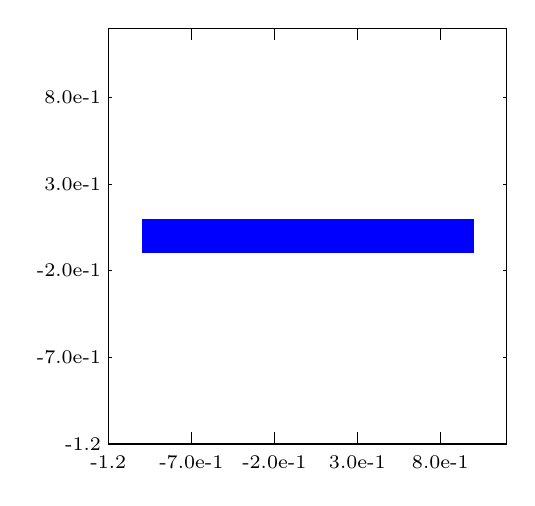
\begin{tikzpicture}[scale = 6,font=\scriptsize]
\draw (0.1148,0.085) rectangle (0.958,0.965);
\foreach \x/\label in {0.1148/-1.2,0.290466/-7.0e-1,0.466133/-2.0e-1,0.6418/3.0e-1,0.817466/8.0e-1} {
  \foreach \y in {0.94,0.085} \draw (\x,\y) -- (\x,\y+0.025);
  \node [below] at (\x,0.08) {\label};
}
\foreach \y/\label in {0.0849996/-1.2,0.268333/-7.0e-1,0.451666/-2.0e-1,0.635/3.0e-1,0.818333/8.0e-1} {
  \foreach \x in {0.951,0.1148} \draw (\x,\y) -- (\x+0.007,\y);
  \node [left] at (0.12,\y) {\label};
}
\fill [blue] (0.185067,0.488333) rectangle (0.887733,0.561667);
\end{tikzpicture}
\hspace{1cm}
% polygon
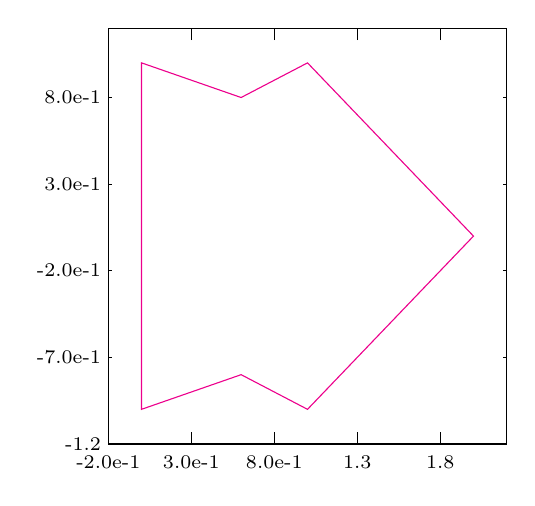
\begin{tikzpicture}[scale = 6,font=\scriptsize]
\draw (0.1148,0.085) rectangle (0.958,0.965);
\foreach \x/\label in {0.1148/-2.0e-1,0.290466/3.0e-1,0.466133/8.0e-1,0.6418/1.3,0.817466/1.8} {
  \foreach \y in {0.94,0.085} \draw (\x,\y) --(\x,\y+0.025);
  \node [below] at (\x,0.08) {\label};
}
\foreach \y/\label in {0.0849996/-1.2,0.268333/-7.0e-1,0.451666/-2.0e-1,0.635/3.0e-1,0.818333/8.0e-1} {
  \foreach \x in {0.951,0.1148} \draw (\x,\y) --(\x+0.007,\y);
  \node [left] at (0.12,\y) {\label};
}
\draw [magenta] (0.185067,0.891667) -- (0.185067,0.158333) -- (0.395867,0.231667) -- (0.5364,0.158333) -- (0.887733,0.525) -- (0.5364,0.891667) -- (0.395867,0.818333) -- cycle;
\end{tikzpicture}
\\[8mm]
% ellipse
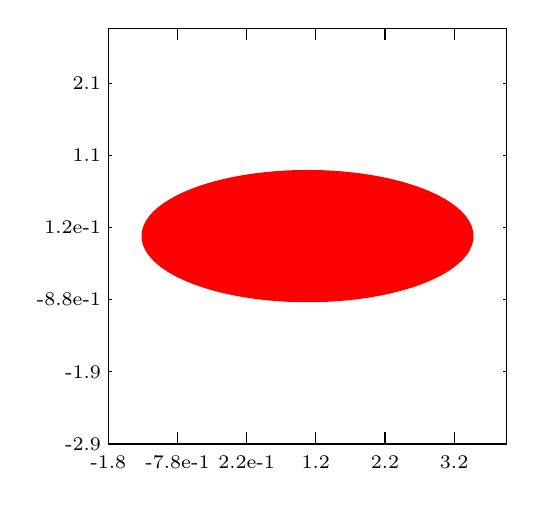
\begin{tikzpicture}[scale = 6,font=\scriptsize]
\draw (0.1148,0.085) rectangle (0.958,0.965);
\foreach \x/\label in {0.1148/-1.8,0.261189/-7.8e-1,0.407578/2.2e-1,0.553966/1.2,0.700355/2.2,0.846744/3.2} {
  \foreach \y in {0.94,0.085} \draw (\x,\y) --(\x,\y+0.025);
  \node [below] at (\x,0.08) {\label};
}
\foreach \y/\label in {0.0849996/-2.9,0.237777/-1.9,0.390555/-8.8e-1,0.543333/1.2e-1,0.696111/1.1,0.848888/2.1} {
  \foreach \x in {0.951,0.1148} \draw (\x,\y) --(\x+0.007,\y);
  \node [left] at (0.12,\y) {\label};
}
\fill [red] (0.5364,0.525) circle [x radius=0.351333,y radius=0.14];
\end{tikzpicture}
\hspace{1cm}
% ring
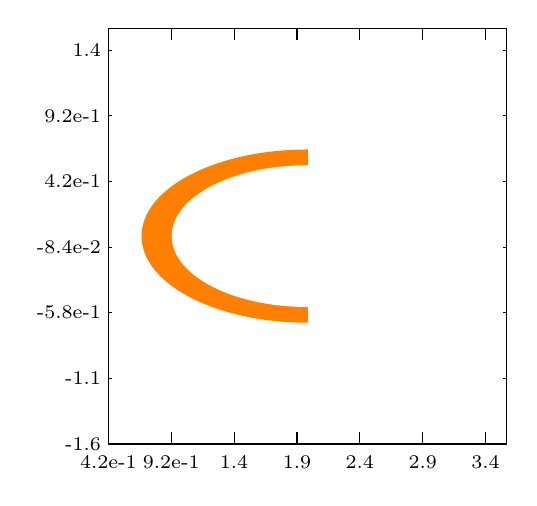
\begin{tikzpicture}[scale = 6,font=\scriptsize]
\draw (0.1148,0.085) rectangle (0.958,0.965);
\foreach \x/\label in {0.1148/4.2e-1,0.247881/9.2e-1,0.380962/1.4,0.514043/1.9,0.647123/2.4,0.780204/2.9,0.913285/3.4} {
  \foreach \y in {0.94,0.085} \draw (\x,\y) --(\x,\y+0.025);
  \node [below] at (\x,0.08) {\label};
}
\foreach \y/\label in {0.0849996/-1.6,0.223888/-1.1,0.362777/-5.8e-1,0.501666/-8.4e-2,0.640555/4.2e-1,0.779444/9.2e-1,0.918333/1.4} {
  \foreach \x in {0.951,0.1148} \draw (\x,\y) --(\x+0.007,\y);
  \node [left] at (0.12,\y) {\label};
}
\fill [color=orange] (0.5364,0.525) circle [x radius=0.351333,y radius=0.183333];
\fill [color=white] (0.5364,0.525) circle [x radius=0.287455,y radius=0.15];
\fill [color=white] (0.5364,0.158333) rectangle (0.9,0.784272);
\end{tikzpicture}
\caption{\label{fig:rg}Sample regions defined via the \ident{RG} class: interval (top left), polygon (top right), ellipse (bottom left), and ring (bottom right). These plots can be generated at run time by adding the command-line option \texttt{-rg\_view draw}.}
\end{figure}

Sometimes it is useful to specify the complement of a certain region, e.g., the part of the complex plane outside an ellipse. This can be achieved with
	\findex{RGSetComplement}
	\begin{Verbatim}[fontsize=\small]
        RGSetComplement(RG rg,PetscBool flg)
	\end{Verbatim}
or in the command line with \Verb!-rg_complement!.

By default, a newly created \ident{RG} object that is not set a type nor parameters must represent the whole complex plane (the same as \texttt{RGINTERVAL} with values $[-\infty,+\infty]\times[-\infty,+\infty]$). We call this the \emph{trivial} region, and provide a function to test this situation:
	\findex{RGIsTrivial}
	\begin{Verbatim}[fontsize=\small]
        RGIsTrivial(RG rg,PetscBool *trivial)
	\end{Verbatim}

Another useful operation is to check whether a given point of the complex plane is inside the region or not:
	\findex{RGCheckInside}
	\begin{Verbatim}[fontsize=\small]
        RGCheckInside(RG rg,PetscInt n,PetscScalar *ar,PetscScalar *ai,PetscInt *inside)
	\end{Verbatim}
Note that the point is represented as two \texttt{PetscScalar}'s, similarly to eigenvalues in \slepc.

\begin{table}
\centering
{\small \begin{tabular}{lll}
                       &                     & {\footnotesize Options} \\
Region Type            & \ident{RGType}      & {\footnotesize Database Name}\\\hline
(Generalized) Interval & \texttt{RGINTERVAL} & \texttt{interval} \\
Polygon                & \texttt{RGPOLYGON}  & \texttt{polygon} \\
Ellipse                & \texttt{RGELLIPSE}  & \texttt{ellipse} \\
Ring                   & \texttt{RGRING}     & \texttt{ring} \\\hline
\end{tabular} }
\caption{\label{tab:rg}Regions available as \ident{RG} objects.}
\end{table}

%---------------------------------------------------
\section{Directory Structure}

	The directory structure of the \slepc software is very similar to that in \petsc. The root directory of \slepc contains the following directories:
\begin{description}
\item[\texttt{lib/slepc/conf}] - Directory containing the base \slepc makefile, to be included in application makefiles.
\item[\texttt{config}] - \slepc configuration scripts.
\item[\texttt{docs}] - All documentation for \slepc, including this manual. The subdirectory \texttt{manualpages} contains the on-line manual pages of each \slepc routine.
\item[\texttt{include}] - All include files for \slepc. The following subdirectories exist:
\begin{description}
\setlength{\itemsep}{0mm}
\item[\texttt{slepc/finclude}] - include files for Fortran programmers.
\item[\texttt{slepc/private}] - include files containing implementation details, for developer use only.
\end{description}
\item[\texttt{share/slepc}] - Common files, including:
\begin{description}
\setlength{\itemsep}{0mm}
\item[\texttt{datafiles}] - data files used by some examples.
%\item[\texttt{matlab}] - Matlab interface and examples.
\end{description}
\item[\texttt{src}] - The source code for all \slepc components, which currently includes:
\begin{description}
\setlength{\itemsep}{0mm}
\item[\texttt{sys}] - system-related routines and auxiliary classes \texttt{bv}, \texttt{ds}, \texttt{fn}, \texttt{rg}, \texttt{st}.
\item[\texttt{eps}] - eigenvalue problem solver.
\item[\texttt{svd}] - singular value decomposition solver.
\item[\texttt{pep}] - polynomial eigenvalue problem solver.
\item[\texttt{nep}] - nonlinear eigenvalue problem solver.
\item[\texttt{mfn}] - matrix function.
\item[\texttt{lme}] - linear matrix equations.
\end{description}
\item[\texttt{\$PETSC\_ARCH}] - For each value of \ident{PETSC\_ARCH}, a directory exists containing files generated during installation of that particular configuration. The following subdirectories exist:
\begin{description}
\setlength{\itemsep}{0mm}
\item[\texttt{lib}] - all the generated libraries.
\item[\texttt{lib/slepc/conf}] - configuration parameters and log files.
\item[\texttt{include}] - automatically generated include files, such as Fortran 90 \texttt{*.mod} files.
\end{description}
\end{description}

Each \slepc source code component directory has the following subdirectories:
\begin{description}
\item[\texttt{interface}] - The calling sequences for the abstract interface to the components. Code here does not know about particular implementations.
\item[\texttt{impls}] - Source code for the different implementations.
\item[\texttt{tutorials}] - Example programs intended for learning to use \slepc.
\item[\texttt{tests}] - Example programs used by testing scripts.
\end{description}

%---------------------------------------------------
%\section{Auxiliary Components}
%\label{sec:aux}

%The previous section includes a list of subdirectories, each of them representing a \slepc component. Most of these components have been treated in previous chapters. Here we include a brief report about two auxiliary components, \ident{BV} and \ident{DS}, that are not normally required by final users, but provide important operations to high level solvers such \ident{EPS}.

%\subsection{BV: Basis Vectors}

%\subsection{DS: Direct Solver (or Dense System)}

%---------------------------------------------------
\section{Wrappers to External Libraries}
\label{sec:wrap}

	\slepc interfaces to several external libraries for the solution of eigenvalue problems. This section provides a short description of each of these packages as well as some hints for using them with \slepc, including pointers to the respective websites from which the software can be downloaded. The description may also include method-specific parameters, that can be set in the same way as other \slepc options, either procedurally or via the command-line.

	In order to use \slepc together with an external library such as \arpack, one needs to do the following.
	\begin{enumerate}
	\item Install the external software, with the same compilers and MPI that will be used for \petsc/\slepc.
	\item Enable the utilization of the external software from \slepc by specifying configure options as explained in \S\ref{sec:opt-inst}.
 	\item Build the \slepc libraries.
	\item Use the runtime option \Verb!-eps_type <type>! to select the solver.
	\end{enumerate}

	Exceptions to the above rule are \lapack, which should be enabled during \petsc's configuration, and \blopex, that must be installed with \Verb!--download-blopex! in \slepc's configure. Other packages also support the download option.

\subsection*{\underline{\lapack}}
	\begin{description}
	\setlength{\itemsep}{0pt}
	\item[References.]\citep{Anderson:1992:LUG}.
	\item[Website.] \url{http://www.netlib.org/lapack}.
	\item[Version.] 3.0 or later.
	\item[Summary.] \lapack\ (Linear Algebra PACKage) is a software package for the solution of many different dense linear algebra problems, including various types of eigenvalue problems and singular value decompositions.

	\slepc explicitly creates the operator matrix in dense form and then the appropriate \lapack driver routine is invoked. Therefore, this interface should be used only for testing and validation purposes and not in a production code. The operator matrix is created by applying the operator to the columns of the identity matrix.

	\item[Installation.]
	The \slepc interface to \lapack can be used directly. If \slepc's configure script complains about missing \lapack functions, then configure \petsc with option \texttt{-{}-download-f2cblaslapack}.
	\end{description}

\subsection*{\underline{\arpack}}
	\begin{description}
	\setlength{\itemsep}{0pt}
	\item[References.]\citep{Lehoucq:1998:AUG}, \citep{Maschhoff:1996:PEP}.
	\item[Website.] \url{http://www.caam.rice.edu/software/ARPACK}.
	\item[Version.] Release 2 (plus patches).
	\item[Summary.] \arpack\ (ARnoldi PACKage) is a software package for the computation of a few eigenvalues and corresponding eigenvectors of a general $n\times n$ matrix $A$. It is most appropriate for large sparse or structured matrices, where structured means that a matrix-vector product $w \leftarrow Av$ requires order $n$ rather than the usual order $n^2$ floating point operations.
	
	\arpack\ is based upon an algorithmic variant of the Arnoldi process called the Implicitly Restarted Arnoldi Method (IRAM). When the matrix $A$ is symmetric it reduces to a variant of the Lanczos process called the Implicitly Restarted Lanczos Method (IRLM). These variants may be viewed as a synthesis of the Arnoldi/Lanczos process with the Implicitly Shifted QR technique that is suitable for large scale problems.

	It can be used for standard and generalized eigenvalue problems, both in real and complex arithmetic. It is implemented in Fortran 77 and it is based on the reverse communication interface. A parallel version, \parpack, is available with support for both MPI and BLACS.
	\item[Installation.]
	To install from the original website: first of all, unpack \texttt{arpack96.tar.gz} and also the patch file \texttt{patch.tar.gz}. If you plan to use the parallel version, extract also the contents of the file \texttt{parpack96.tar.gz} together with the patches \texttt{ppatch.tar.gz} (make sure you delete any \texttt{mpif.h} files that could exist in the directory tree). After setting all the directories, modify the \texttt{ARmake.inc} file and then compile the software with \texttt{make all}. It is recommended that \arpack is installed with its own \lapack version since it may give unexpected results with more recent versions of \lapack.

	Alternatively, one can use the \textsc{arpack-ng} distribution, available in \texttt{github.com}, that supports \texttt{configure}+\texttt{make} for installation. Also, \slepc's \texttt{configure} allows to download this version automatically via the \texttt{-{}-download-arpack} option.

	It is possible to configure \slepc with the serial version of \arpack. For this, you have to configure \petsc with the option \texttt{-{}-with-mpi=0}.
	\end{description}

\subsection*{\underline{\primme}}
	\begin{description}
	\setlength{\itemsep}{0pt}
	\item[References.]\citep{Stathopoulos:2010:PMS}.
	\item[Website.] \url{http://www.cs.wm.edu/~andreas/software}.
	\item[Version.] 3.0.
	\item[Summary.] \primme (PReconditioned Iterative MultiMethod Eigensolver) is a C library for finding a number of eigenvalues and their corresponding eigenvectors of a real symmetric (or complex Hermitian) matrix. This library provides a multimethod eigensolver, based on Davidson/Jacobi-Davidson. Particular methods include GD+1, JDQMR, and LOBPCG. It supports preconditioning as well as the computation of interior eigenvalues.
	\item[Installation.] Type \texttt{make lib} after customizing the file \texttt{Make\_flags} appropriately. Alternatively, the \texttt{-{}-download-primme} option is also available in \slepc's \texttt{configure}.
	\item[Specific options.] Since PRIMME contains preconditioned solvers, the \slepc interface uses \ident{STPRECOND}, as described in \ref{sec:precond}.

The \slepc interface to this package allows the user to specify the maximum allowed block size with the function \ident{EPSPRIMMESetBlockSize} or at run time with the option \Verb!-eps_primme_blocksize <size>!.
For changing the particular algorithm within \primme, use the function \ident{EPSPRIMMESetMethod}.

\primme also provides a solver for the singular value decomposition that is interfaced in \slepc's \ident{SVD}, see chapter \ref{cap:svd}.
	\end{description}

\subsection*{\underline{\blzpack}}
	\begin{description}
	\setlength{\itemsep}{0pt}
	\item[References.]\citep{Marques:1995:BDU}.
	\item[Website.] \url{https://crd.lbl.gov/\~osni/\#Software}.
	\item[Version.] 04/00.
	\item[Summary.] \blzpack\ (Block LancZos PACKage) is a standard Fortran 77 implementation of the block Lanczos algorithm intended for the solution of the standard eigenvalue problem $Ax=\mu x$ or the generalized eigenvalue problem $Ax=\mu Bx$, where A and B are real, sparse symmetric matrices. The development of this eigensolver was motivated by the need to solve large, sparse, generalized problems from free vibration analysis in structural engineering. Several upgrades were performed afterwards aiming at the solution of eigenvalue problems from a wider range of applications.

	\blzpack\ uses a combination of partial and selective re-orthogonalization strategies. It can be run in either sequential or parallel mode, by means of MPI or PVM interfaces, and it uses the reverse communication strategy.
	\item[Installation.] For the compilation of the \texttt{libblzpack.a} library, first check the appropriate architecture file in the directory \texttt{sys/MACROS} and then type \texttt{creator -mpi}.
	\item[Specific options.] The \slepc interface to this package allows the user to specify the block size with the function \ident{EPSBlzpackSetBlockSize} or at run time with the option \Verb!-eps_blzpack_! \Verb!blocksize <size>!. Also, the function \ident{EPSBlzpackSetNSteps} can be used to set the maximum number of steps per run (also with \Verb!-eps_blzpack_nsteps!).
	\end{description}

\subsection*{\underline{\trlan}}
	\begin{description}
	\setlength{\itemsep}{0pt}
	\item[References.]\citep{Wu:2000:TLM}.
	\item[Website.] \url{https://crd.lbl.gov/\~kewu/trlan.html}.
	\item[Version.] 201009.
	\item[Summary.] This package provides a Fortran 90 implementation of the dynamic thick-restart Lanczos algorithm. This is a specialized version of Lanczos that targets only the case in which one wants both eigenvalues and eigenvectors of a large real symmetric eigenvalue problem that cannot use the shift-and-invert scheme. In this case the standard non-restarted Lanczos algorithm requires to store a large number of Lanczos vectors, what can cause storage problems and make each iteration of the method very expensive.

	\trlan{} requires the user to provide a matrix-vector multiplication routine. The parallel version uses MPI as the message passing layer.
	\item[Installation.] To install this package, it is necessary to have access to a Fortran 90 compiler. The compiler name and the options used are specified in the file called \texttt{Make.inc}. To generate the library, type \texttt{make plib} in the \texttt{TRLan} directory. Alternatively, the \texttt{-{}-download-trlan} option is also available in \slepc's \texttt{configure}.

	It is possible to configure \slepc with the serial version of \trlan (built with \texttt{make lib}). For this, you have to configure \petsc with the option \texttt{-{}-with-mpi=0}.
	\end{description}

\subsection*{\underline{\blopex}}
	\begin{description}
	\setlength{\itemsep}{0pt}
	\item[References.]\citep{Knyazev:2007:BLO}.
	\item[Website.] \url{https://github.com/lobpcg/blopex}.
	\item[Summary.] \blopex is a package that implements the Locally Optimal Block Preconditioned Conjugate Gradient (LOBPCG) method for computing several extreme eigenpairs of symmetric positive generalized eigenproblems. Numerical comparisons suggest that this method is a genuine analog for eigenproblems of the standard preconditioned conjugate gradient method for symmetric linear systems.
	\item[Installation.] In order to use \blopex from \slepc, it necessary to install it during \slepc's configuration: \Verb!./configure --download-blopex!.
	\item[Specific options.] Since BLOPEX contains preconditioned solvers, the \slepc interface uses \ident{STPRECOND}, as described in \ref{sec:precond}.
	\end{description}

\subsection*{\underline{\elemental}}
	\begin{description}
	\setlength{\itemsep}{0pt}
	\item[References.]\citep{Poulson:2013:ELE}.
	\item[Website.] \url{https://github.com/elemental/Elemental}.
	\item[Summary.] \elemental is distributed-memory, arbitrary-precision, dense and sparse-direct linear algebra package. It contains eigensolvers for dense Hermitian eigenvalue problems.
	\item[Installation.] For using \elemental from \slepc it is necessary to select it during configuration of \petsc.
	\end{description}

\subsection*{\underline{\feast}}
	\begin{description}
	\setlength{\itemsep}{0pt}
	\item[References.]\citep{Polizzi:2009:DAS}.
	\item[Website.] \url{http://www.ecs.umass.edu/~polizzi/feast}.
	\item[Summary.] \feast is a numerical library for solving the standard or generalized symmetric eigenvalue problem, and obtaining all the eigenvalues and eigenvectors within a given search interval. It is based on an innovative fast and stable numerical algorithm which deviates fundamentally from the traditional Krylov subspace based iterations or Davidson-Jacobi techniques. The FEAST algorithm takes its inspiration from the density-matrix representation and contour integration technique in quantum mechanics. Latest versions also support non-symmetric problems.
	\item[Installation.] We only support the \feast implementation included in Intel MKL. For using it from \slepc it is necessary to configure \petsc with MKL by adding the corresponding option, e.g., \Verb!--with-blas-lapack-dir=$MKLROOT!.
	\item[Specific options.] The \slepc interface to \feast allows the user to specify the number of contour integration points with the function \ident{EPSFEASTSetNumPoints} or at run time with the option \Verb!-eps_feast_num_points <n>!.
	\end{description}

%---------------------------------------------------
\section{Fortran Interface}
\label{sec:fortran}

	\slepc provides an interface for Fortran programmers, very much like \petsc. As in the case of \petsc, there are slight differences between the C and Fortran \slepc interfaces, due to differences in Fortran syntax. For instance, the error checking variable is the final argument of all the routines in the Fortran interface, in contrast to the C convention of providing the error variable as the routine's return value.

	The following is a Fortran example with fixed-format source. It is the Fortran equivalent of the program given in \S\ref{sec:simpleex} and can be found in \Verb!${SLEPC_DIR}/src/eps/tutorials! (file \texttt{ex1f.F}). It is also possible to use free-format source (see \texttt{ex1f90.F90}).
\MyVerbatimInput{ex1f.F}

%---------------------------------------------------
%\section{Matlab Interface}
%\label{sec:matlab}
%
%Since version 3.2, \slepc includes an interface intended to make most of \slepc's functionality available from Matlab. It is experimental and needs further development, so users planning to use it seriously are recommended to contact the authors. Below are some guidelines for using this interface.
%
%First of all, \petsc must have been configured with the Matlab interface enabled. This can be done as follows (check \petsc documentation for details):
%	\begin{Verbatim}[fontsize=\small]
%	$ ./configure --with-matlab --with-matlab-engine --with-shared-libraries
%	\end{Verbatim}
%
%Once the \petsc and \slepc libraries have been built, one has to set Matlab's path to point to the directories containing Matlab classes: \Verb!$SLEPC_DIR/share/slepc/matlab/classes! and \Verb!$PETSC_DIR/share/slepc/matlab/classes!. Below we show a simple Matlab example (included in \slepc's distribution) that does this, and then solves a simple eigenproblem.
%\MyVerbatimInput{exEPS.m}

